\documentclass[a4paper,12pt]{article}
%%%%%%%%%%%%%%%%%%%%%%%%%%%%%%%%%%%%%%%%%%%%%%%%%%%%%%%%%%%%%%%%%%%%%%%%%%%%%%%%%%%%%%%%%%%%%%%%%%%%%%%%%%%%%%%%%%%%%%%%%%%%%%%%%%%%%%%%%%%%%%%%%%%%%%%%%%%%%%%%%%%%%%%%%%%%%%%%%%%%%%%%%%%%%%%%%%%%%%%%%%%%%%%%%%%%%%%%%%%%%%%%%%%%%%%%%%%%%%%%%%%%%%%%%%%%
\usepackage{eurosym}
\usepackage{vmargin}
\usepackage{framed}
\usepackage{amsmath}
\usepackage{graphics}
\usepackage{epsfig}
\usepackage{subfigure}
\usepackage{fancyhdr}

\setcounter{MaxMatrixCols}{10}
%TCIDATA{OutputFilter=LATEX.DLL}
%TCIDATA{Version=5.00.0.2570}
%TCIDATA{<META NAME="SaveForMode"CONTENT="1">}
%TCIDATA{LastRevised=Wednesday, February 23, 201113:24:34}
%TCIDATA{<META NAME="GraphicsSave" CONTENT="32">}
%TCIDATA{Language=American English}

\pagestyle{fancy}
\setmarginsrb{20mm}{0mm}{20mm}{25mm}{12mm}{11mm}{0mm}{11mm}
\lhead{MA4128} \rhead{Kevin O'Brien} \chead{Logistic Regression} %\input{tcilatex}

\begin{document}


\section{Binary Logistic Regression}
Binary Logistic regression is used to determine the impact of multiple independent variables
presented simultaneously to predict membership of one or other of the two
dependent variable categories.




\subsection{The Hosmer-Lemeshow Test}
%http://www.strath.ac.uk/aer/materials/5furtherquantitativeresearchdesignandanalysis/unit6/goodnessoffitmeasures/

\noindent \textbf{Performing the Hosmer-Lemeshow Goodness-of-Fit Test} 	
\begin{itemize}	
	\item 	
	The Hosmer-Lemeshow test of goodness of fit is not automatically a part of the SPSS logistic regression output. 
	To get this output, we need to go into \textbf{\texttt{options}} and tick the box marked Hosmer-Lemeshow test of goodness of fit. 
\end{itemize}



In our example, this gives us the following output:

\begin{center}
	\begin{tabular}{|c|c|c|c|}
		\hline  Step	& Chi-square&	df 	 & Sig. \\ \hline
		1	 & 142.032	& 6	 &.000 \\ 
		\hline 
	\end{tabular} 
\end{center}


Therefore, our model is significant, suggesting it does not fit the data. However, as we have a sample size of over 13,000, even very small divergencies of the model from the data would be flagged up and cause significance. Therefore, with samples of this size it is hard to find models that are parsimonious (i.e. that use the minimum amount of independent variables to explain the dependent variable) and fit the data. Therefore, other fit indices might be more appropriate.

% Binary Regression : http://teaching.sociology.ul.ie/SSS/lugano/node10.html 
% http://istics.net/pdfs/multivariate.pdf
%---------------------------------------------------------- %
\section{Logistic Regression}
Logistic regression, also called a logit model, is used to model \textbf{dichotomous outcome} variables. 
In the logit model the \textbf{log odds} of the outcome is modeled as a linear combination of the predictor variables.

In logistic regression theory, the predicted dependent variable is a function of the probability that a particular subject will be in one of the categories (for example, the probability that a patient has the disease, given his or her set of scores on the predictor variables).



\subsection{Model Summary Table}


The likelihood function can be thought of as a measure of how well a candidate model fits the data (although that is a very simplistic definition). The AIC criterion is based on the Likelihood function.
The likelihood function of a fitted model is commonly re-expressed as -2LL (i.e. The log of the likelihood times minus 2). The –2LL value from the Model Summary table below is 17.359.



\subsection{Hosmer and Lemeshow  Statistic}
An alternative to model chi square is the Hosmer and Lemeshow test
which divides subjects into 10 ordered groups of subjects and then compares the number
actually in the each group (observed) to the number predicted by the logistic regression
model (predicted). The 10 ordered groups are created based on their estimated probability; those with estimated probability below .1 form one group, and so on, up to those with probability .9 to 1.0.

Each of these categories is further divided into two groups based on the actual observed outcome variable (success, failure). The expected frequencies for each of the cells are obtained from the model. A probability (p) value is
computed from the chi-square distribution with 8 degrees of freedom to test the fit of the logistic model.

If the H-L goodness-of-fit test statistic is greater than .05, as we want for well-fitting models, we fail to reject the null hypothesis that there is no difference between observed and model-predicted values, implying that the model’s estimates fit the data at an acceptable level. That is, well-fitting models show non-significance on the
H-L goodness-of-fit test. This desirable outcome of non-significance indicates that the
model prediction does not significantly differ from the observed.

The H-L statistic assumes sampling adequacy, with a rule of thumb being enough cases so that 95\% of cells (typically, 10 decile groups times 2 outcome categories = 20 cells) have an expected frequency $>$ 5. Our H-L statistic has a significance of .605 which means that it is not statistically significant and therefore our model is quite a
good fit.
\begin{figure}[h!]
	\begin{center}
		% Requires \usepackage{graphicx}
		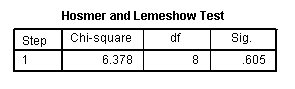
\includegraphics[scale=0.6]{images/Logistic7A}\\
		\caption{Hosmer and Lemeshow Statistic}
	\end{center}
\end{figure}

\begin{figure}[h!]
	\begin{center}
		% Requires \usepackage{graphicx}
		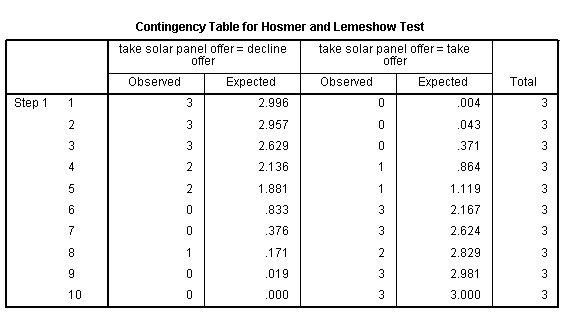
\includegraphics[scale=0.6]{images/Logistic6}\\
		\caption{Hosmer and Lemeshow Table}
	\end{center}
\end{figure}


\section{Model Diagnostics for Logistic Regression}
%http://statistics.ats.ucla.edu/stat/mult_pkg/faq/general/Psuedo_RSquareds.htm

%http://www.strath.ac.uk/aer/materials/5furtherquantitativeresearchdesignandanalysis/unit6/goodnessoffitmeasures/


\section*{The Wald Test}

\begin{itemize}
	\item 	The Wald test is a way of testing the signi®cance of particular explanatory variables in a statistical model. In logistic regression we have a binary outcome variable and one or more explanatory variables. For each explanatory variable in the model there will be an associated parameter.
	\item 	The Wald test, described by Polit (1996) and Agresti (1990), is one of a number of ways of testing whether the parameters associated with a group of
	explanatory variables are zero.
	
	\item 	If for a particular explanatory variable, or group of explanatory variables, the Wald test is significant, then we would conclude that the parameters associated with these variables are not zero, so that the variables should be included in the model. If the Wald test is not significant then these explanatory variables can be omitted from the model. When considering a single explanatory variable, Altman (1991) uses a t-test to check whether the parameter is significant. 
	
	\item 		For a single parameter the Wald statistic is just the square of the t-statistic and so will give exactly equivalent results.
	An alternative and widely used approach to testing the significance of a number of explanatory variables is to use the likelihood ratio test. This is
	appropriate for a variety of types of statistical models. Agresti (1990) argues that the likelihood ratio test is better, particularly if the sample size is small or the parameters are large.
\end{itemize}

\subsection{Logistic Regression}

\[ \pi(x) = \frac{e^{(\beta_0 + \beta_1 x)}} {e^{(\beta_0 + \beta_1 x)} + 1} = \frac {1} {e^{-(\beta_0 + \beta_1 x)} + 1},\]
and

\[g(x) = \ln \frac {\pi(x)} {1 - \pi(x)} = \beta_0 + \beta_1 x ,\]

and

\[\frac{\pi(x)} {1 - \pi(x)} = e^{(\beta_0 + \beta_1 x)}.\]

\subsection{Wald statistic}

Alternatively, when assessing the contribution of individual predictors in a given model, one may examine the significance of the Wald statistic. The Wald statistic, analogous to the t-test in linear regression, is used to assess the significance of coefficients. The Wald statistic is the ratio of the square of the regression coefficient to the square of the standard error of the coefficient and is asymptotically distributed as a chi-square distribution.



\subsection{Wald statistic}
The Wald statistic is commonly used to test the significance of individual logistic regression coefficients for each independent variable (that is, to test the null hypothesis in logistic regression that a particular logit (effect) coefficient is zero). 

The Wald Statistic is the ratio of the unstandardized logit coefficient to its standard error. The Wald statistic and its corresponding p probability level is part of SPSS output in the section \textbf{\textit{Variables in the Equation.}} This corresponds to significance testing of b coefficients in OLS regression. The researcher may well want to drop independents from the model when their effect is not significant by the Wald statistic.
\newpage
%-------------------------------------------%



\subsection{Logistic Regression: Decision Rule}
Our decision rule will take the following form: If the probability of the event is greater than or equal to some threshold, we shall predict that the event will take place. By default, SPSS sets this threshold to .5. While that seems reasonable, in many cases we may want to set it higher or lower than .5.

%---------------------------------------------------------- %

\section{Model Diagnostics for Logistic Regression}
%http://statistics.ats.ucla.edu/stat/mult_pkg/faq/general/Psuedo_RSquareds.htm

%http://www.strath.ac.uk/aer/materials/5furtherquantitativeresearchdesignandanalysis/unit6/goodnessoffitmeasures/

\noindent \textbf{Remark upon ``Steps"}
\begin{itemize}
	\item This table has 1 step. This is because we are entering both variables and at the same
	time providing only one model to compare with the constant model. 
	\item In stepwise logistic regression there are a number of steps listed in the table as each variable is added or
	removed, creating different models. 
	\item The step is a measure of the improvement in the
	predictive power of the model since the previous step. 
	\item I will revert to this next class.
\end{itemize}

\subsection{Model Summary Table}

\begin{itemize}
	\item The likelihood function can be thought of as a measure of how well a candidate model fits the data (although that is a very simplistic definition). 
	\item Later on in the course, we will meet the AIC Function. The AIC criterion is based on the Likelihood function.
	\item The likelihood function of a fitted model is commonly re-expressed as $-2LL$ (i.e. The log of the likelihood times minus 2). The –2LL value from the Model Summary table below is 17.359.
	\item It is not immediately clear how to interpret $-2LL$ yet. However this measure is useful in comparing various candidate models, and is therefore used in \textbf{\textit{Variable Selection Procedure}}, such as backward and forward selection.
\end{itemize}

\begin{figure}[h!]
	\centering
	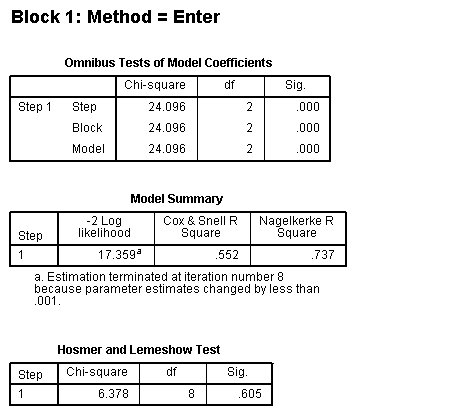
\includegraphics[width=0.9\linewidth]{images/Logistic5}
\end{figure}










	
	The Wald Test is a statistical test used to determine whether an effect exists or not,
	
	It tests whether an independent variable has a statistically significant relationship with a dependent variable.
	
	It is used in a great variety of different models including models for dichotomous variables and model for continuous
	variables.
	
	\begin{itemize}
		\item $\hat{\theta}$ Maximum likelihood estimate of the parameter of interest $\theta$
		\item $\theta_o$ Proposed value.
		This is an assumption of the fact that the differences between $\hat{\theta}$ and $\theta_o$ is normal.
		
		Univariate case
		\[ \frac{(\hat{\theta} - \theta_o )^2}{\mbox{var}(\hat{\theta})} \sim \chi^2 \]
		\[ \frac{(\hat{\theta} - \theta_o )^2}{\mbox{s.e.}(\hat{\theta})} \sim \mbox{Normal} \]
	\end{itemize}	
	The likelihood ratio test is also used to determine whether an effect exists.
	]
\newpage



\subsection*{Wald Test}

The Wald Test is a statistical test used to determine whether an effect exists or not,

It tests whether an independent variable has a statistically significant relationship with a dependent variable.

It is used in a great variety of different models including models for dichotomous variables and model for continuous
variables.

\begin{itemize}
	\item $\hat{\theta}$ Maximum likelihood estimate of the parameter of interest $\theta$
	\item $\theta_o$ Proposed value.
	This is an assumption of the fact that the differences between $\hat{\theta}$ and $\theta_o$ is normal.
	
	Univariate case
	\[ \frac{(\hat{\theta} - \theta_o )^2}{\mbox{var}(\hat{\theta})} \sim \chi^2 \]
	\[ \frac{(\hat{\theta} - \theta_o )^2}{\mbox{s.e.}(\hat{\theta})} \sim \mbox{Normal} \]
\end{itemize}	
The likelihood ratio test is also used to determine whether an effect exists.


%============================================================================================%


	\section{Wald statistic}
\begin{itemize}
	\item Alternatively, when assessing the contribution of individual predictors in a given model, one may examine the significance of the Wald statistic. The Wald statistic, analogous to the t-test in linear regression, is used to assess the significance of coefficients. 
 

	
	\item The Wald statistic is the ratio of the square of the regression coefficient to the square of the standard error of the coefficient and is asymptotically distributed as a chi-square distribution.
	
	\[W_j = \frac{B^2_j} {SE^2_{B_j}}\]
	
	\item Although several statistical packages (e.g., SPSS, SAS) report the Wald statistic to assess the contribution of individual predictors, the Wald statistic has limitations. 
	\item When the regression coefficient is large, the standard error of the regression coefficient also tends to be large increasing the probability of Type-II error. 
	
	\item The Wald statistic is the ratio of the square of the regression coefficient to the square of the standard error of the coefficient and is asymptotically distributed as a chi-square distribution.
	
	\item The Wald statistic also tends to be biased when data are sparse.
\end{itemize}
% Wald Test?
%--------------------------------------------------------%
\begin{figure}[h!]
	\centering
	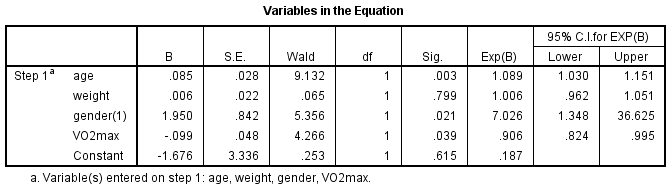
\includegraphics[width=0.7\linewidth]{images/waldtest}
	\caption{}
	\label{fig:waldtest}
\end{figure}

\subsection{The Wald Test}





	\section{Wald statistic}
	\begin{itemize}
		\item Alternatively, when assessing the contribution of individual predictors in a given model, one may examine the significance of the Wald statistic. The Wald statistic, analogous to the t-test in linear regression, is used to assess the significance of coefficients. 
		

				\item The Wald statistic is the ratio of the square of the regression coefficient to the square of the standard error of the coefficient and is asymptotically distributed as a chi-square distribution.
		
		\[W_j = \frac{B^2_j} {SE^2_{B_j}}\]
		
		\item Although several statistical packages (e.g., SPSS, SAS) report the Wald statistic to assess the contribution of individual predictors, the Wald statistic has limitations. 
		\item When the regression coefficient is large, the standard error of the regression coefficient also tends to be large increasing the probability of Type-II error. 
				
		\item The Wald statistic is the ratio of the square of the regression coefficient to the square of the standard error of the coefficient and is asymptotically distributed as a chi-square distribution.
		
		\item The Wald statistic also tends to be biased when data are sparse.
	\end{itemize}

%---------------------------------------------------------- %



%-------------------------------------------------------%

\subsection{Hosmer-Lemeshow Goodness-of-Fit Test}
\begin{framed}
	\begin{itemize}
		\item The Hosmer-Lemeshow Goodness-of-Fit
		test tells us whether we have constructed a valid overall model or not, and is an alternative to model chi square procedure.
		\item If the model is a good fit to the data then the Hosmer-Lemeshow Goodness-of-Fit test should have an associated p-value greater than 0.05.
	\end{itemize} 
\end{framed}
If the H-L goodness-of-fit test statistic is greater than .05, as we want for well-fitting models, we fail to reject the null hypothesis that there is no difference between observed and model-predicted values, implying that the model’s estimates fit the data at an acceptable level. That is, well-fitting models show non-significance on the
H-L goodness-of-fit test. This desirable outcome of non-significance indicates that the
model prediction does not significantly differ from the observed.
%---------------------------------------------------------- %

\subsection{Computing the Hosmer and Lemeshow Test Statistic}

\begin{itemize}
	\item The Hosmer and Lemeshow test
	divides subjects into 10 ordered groups of subjects and then compares the number
	actually in the each group (observed) to the number predicted by the logistic regression
	model (predicted). 
	\item The 10 ordered groups are created based on their estimated probability; those with estimated probability below .1 form one group, and so on, up to those with probability .9 to 1.0.
	\item 
	Each of these categories is further divided into two groups based on the actual observed outcome variable (success, failure). The expected frequencies for each of the cells are obtained from the model. A probability (p) value is
	computed from the chi-square distribution with 8 degrees of freedom to test the fit of the logistic model.
	
\end{itemize}
\begin{figure}[h!]
	\begin{center}
		% Requires \usepackage{graphicx}
		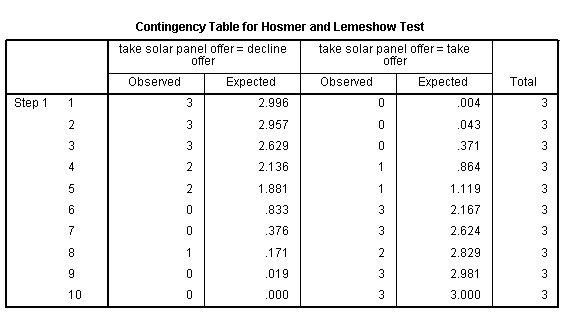
\includegraphics[scale=0.6]{images/Logistic6}\\
		\caption{Hosmer and Lemeshow Table}
	\end{center}
\end{figure}

\subsection{Sample Adequacy}

The H-L statistic assumes sampling adequacy, with a rule of thumb being enough cases so that 95\% of cells (typically, 10 decile groups times 2 outcome categories = 20 cells) have an expected frequency $>$ 5. Our H-L statistic has a significance of .605 which means that it is not statistically significant and therefore our model is quite a
good fit.
\begin{figure}[h!]
	\begin{center}
		% Requires \usepackage{graphicx}
		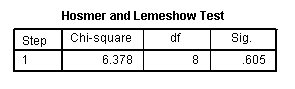
\includegraphics[scale=0.6]{images/Logistic7A}\\
		\caption{Hosmer and Lemeshow Statistic}
	\end{center}
\end{figure}





\end{document}
